\section{Modellierung}
\label{sec:modellierung}

\subsection{Erzeugung von Antwortspektren}

* Variation der Eigenfrequenz

* Gleichung

* Zeitschrittverfahren

\subsection{Erweitertes Modell}

Für die Erzeugung der Isolationsspektren wird hier das System um den Isolator erweitert und als Zweimassenschwinger (\cref{fig:vkm}) betrachtet.
Wobei der obere Schwinger die aufgehende Struktur ($s$) und der untere Schwinger den Isolator ($i$) samt des steifen Kellergeschosses beschreiben soll.

\begin{figure}[ht]
    \centering
    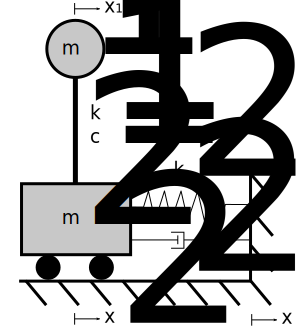
\includegraphics[width=0.5\textwidth]{voigt-kelvin-model.png}
    \caption{Voigt-Kelvin-Modell}
    \label{fig:vkm}
\end{figure}

Unter Annahme der Linearität können die Systeme getrennt betrachtet werden. Am System der Struktur wird durch Parameter Sweeps das Antwortspektrum berechnet. Da der untere Teil des Systems dabei unverändert bleibt kann anschließend durch Komposition das Isolationsspektrum ermittelt werden.
Da das Antwortspektrum für Einmassenschwinger bereits bekannt ist, kann die Betrachtung des Gesamtsystems und eine aufwändige Zeitschrittanalyse entfallen.

\subsection{Bewegungsgleichung}

Die Bewegungsgleichung (siehe auch \cite{Kramer} (S. 92, Gl. 7.3)) für das System des Isolators ist durch

\begin{equation}\label{eq:bewegungsgleichung}
m_i \cdot \ddot x(t) + c_i^* \cdot \dot x(t) + k_i^* \cdot x(t) = 0
\end{equation}

gegeben.

\pagebreak

\section{Betrachtung als Übertragungsfunktion}
\label{sec:ubertragungsfunktion}

\begin{equation} \label{laplace}
F(s) = \int_{0}^{\infty} f(t)e^{-st}dt
\end{equation}

Umformung von (\cref{eq:bewegungsgleichung}) von t in s Domain

\begin{equation} \label{laplace1}
F(s) = m_i \cdot s^2 \cdot x(s) + c_i^* \cdot s \cdot x(s) + k_i^* \cdot x(s)
\end{equation}

Somit ergibt sich die Übertragungsfunktion zu

\begin{equation} \label{laplace2}
G(s)=\frac{X(s)}{F(s)} = \frac{1}{m_i \cdot s^2 + c_i^* \cdot s + k_i^*}
\end{equation}

Die Polstellen ergeben sich zu

\begin{equation} \label{laplace-pole}
s_{1,2} = \frac{-c_i^* \pm \sqrt{(c_i^*)^2 - 4m_ik_i^*}}{2m_i}
\end{equation}

\begin{equation} \label{laplace3}
G(s)=\frac{1}{(s-s_1)(s-s_2)}
\end{equation}

\begin{equation} \label{laplace-attan}
|G(i\omega)|
\end{equation}

* Laplace Transfomration

* Filterfunktion

* Filtern des Spektrums

\pagebreak

\section{Vergleich zum Zweimassenschwinger}
\label{sec:vergleich}

Anahand eines Beispiels soll in einer Handrechnung an einem einfachen System zunächst die auf die aufgehende Struktur wirkende Gesamterdbebenkraft $F_b$ mittels des Isolationsspektrums ermittelt werden und anschließend mit den Ergebnissen einer Berechnung am Zweimassenschwinger verglichen werden.

\begin{figure}[ht]
    \centering
    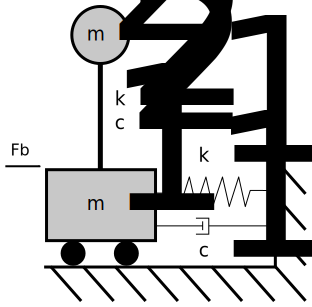
\includegraphics[width=0.5\textwidth]{2MS_beispiel.png}
    \caption{Zweimassenschwinger}
    \label{fig:2ms}
\end{figure}

Die Dämpfung beträgt $c_1 = c_2 = 5\%$, die Masse des Kellergeschosses $m_1 = 0.2 MN/s^2/m$ mit einer Steifigkeit von $k_1 = 5 MN/m$ und die Masse der aufgehenden Struktur $m_2 = 1 MN/s^2/m$ mit einer Steifigkeit von $k_2 = 45 MN/m$.

\subsection{Bemessungsspektrum}

Für dieses Beispiel wird ein Antwortspektrum aus dem Raum Karlsruhe herangezogen. Damit ergibt sich eine Bodenbeschleunigung in der Erdbebenzone 1 von $a_g = 0.4 m/s^2$ und die Baugrundklasse C-S mit den Kontrollperioden $T_B$, $T_C$, $T_D$ und Untergrundparameter $S$:

\begin{align*}
S &= 0.75 s\\
T_B &= 0.1 s\\
T_C &= 0.5 s\\
T_D &= 2.0 s
\end{align*}

Der Bedeutungsbeiwert wird mit $\gamma_1 = 1.0$ für gewöhnliche Bauten mit Bedeutungsklasse II, der Verstärkungsbeiwert der Spektralbeschleunigung mit $\beta_0 = 2.5$ für eine viskose Dämpfung von 5\% und der Verhaltensbeiwert für Duktilitätsklasse 1 mit $q = 1.5$ angesetzt.
Daraus ergibt sich das Bemessungsspektrum zu \cref{fig:Bemessungsspektrum}.

\begin{figure}[ht] 
    \centering
    \includegraphics[width=0.9\textwidth]{AWS_beispiel.png}
    \caption{Bemessungsspektrum}
    \label{fig:Bemessungsspektrum}
\end{figure}

\subsection{Betrachtung mit Isolationsspektrums}

Die Eigenfrequenz der Struktur ergibt sich zu

\begin{align*}
\omega &= \sqrt{\frac{k_2}{m_2}} = \sqrt{\frac{45}{1}}\\
       &= 6.708 s^{-1}
\end{align*}

\begin{align*}
T &= \frac{2 \cdot \pi}{\omega} = \frac{2 \cdot \pi}{6.708}\\
  &= 0.936 s
\end{align*}

und eine Beschleunigung von

\begin{align*}
S_d(T) &= a_g \cdot \gamma_1 \cdot S \cdot \frac{\beta_0}{q} \cdot \frac{T_C}{T}\\
S_d(0.936) &= 0.4 \cdot 1.0 \cdot 0.75 \cdot \frac{2.5}{1.5} \cdot \frac{0.5}{0.936}\\
           &= 0.277 m/s^2
\end{align*}

Die Übertragungsfunktion für den hier gegebenen Isolator lautet:

\begin{align*}
G(s) &= \frac{1}{m_1 \cdot s^2 + c_1 \cdot s + k_1}\\
     &= \frac{1}{0.2 \cdot s^2 + 0.05 \cdot s + 5}
\end{align*}

Um die Amplitude zu erhalten wird der Laplace-Faktor $s$ bestimmt und der Betrag der Übertragungsfunktion ermittelt.

\begin{align*}
s &= i \cdot \omega\\
  &= i \cdot 6.708\\
  &= 6.708i
\end{align*}

\begin{align*}
|G(6.708i)| &= |\frac{1}{0.2 \cdot 6.708i^2 + 0.05 \cdot 6.708i + 5}|\\
            &= 0.208
\end{align*}

Die an der Struktur wirkende Gesamterdbebenkraft $F_b$ ergibt sich somit zu:

\begin{align*}
F_b &= |G(s)| \cdot S_d(T) \cdot m_2\\
    &= 0.208 \cdot 0.277 m/s^2 \cdot 1 MN/s^2/m\\
    &= \underline{\underline{0.0576 MN}}
\end{align*}

\subsection{Betrachtung am Zweimassenschwinger}

Bei der Betrachtung des Zweimassenschwingers kann vereinfacht angenommen werden, dass der weiche Isolator die Eigentform dominiert \cite{AKK} und sich die Eigenfrequenz des Gesamtsystems somit zu

\begin{align*}
\omega_1 &= \sqrt{\frac{k_1}{m_1 + m_2}}\\
         &= \sqrt{\frac{5}{1.0 + 0.2}}\\
         &= 2.041 s^{-1}
\end{align*}

\begin{align*}
T_1 &= \frac{2 \cdot \pi}{\omega} = \frac{2 \cdot \pi}{2.041}\\
    &= 3.078 s
\end{align*}

ergibt. Die auf die Struktur wirkende Gesamterdbebenkraft $F_b$ ist dann:

\begin{align*}
F_b &= S_d(T) \cdot m_2\\
    &= 0.053 m/s^2 \cdot 1 MN/s^2/m\\
    &= \underline{\underline{0.053 MN}}
\end{align*}

Damit liegt die Abweichung der beiden Ansätze in dem Fall bei $0.0576/0.053=1.0945$, also ungefähr $9.5\%$.

\pagebreak

\section{Grenzfälle}
\label{sec:grenzfalle}

*2MS mit Beteiligungsfaktor erklären

*Sweeps

*Abweichung durch Schwebung/Beteiligung 2. Feder erklären

\pagebreak

\section{Nichtlinearitäten und Ansätze zur Linearisierung}
\label{sec:nichtlinearitaten}

*Huber

\pagebreak